\subsection{RQ3: Effectiveness across Task Complexity}
\label{sec:rq3-complexity}
\textbf{RQ3. How does the effectiveness of design-centered generation vary with project and embedded-system complexity?}

\paragraph{From peripheral tasks to coordinated applications.}
We hold the generation model fixed to DeepSeek-V4-Pro and compare \textsc{EmbedDev} with all four RQ1 baselines across six tasks. The range includes two authored GPIO tasks, one control module derived from a project example, and the three multi-component application tasks from RQ1. Table~\ref{tab:rq3-profiles} describes their interface scale and coordination demands. The ordering follows these task groups; neither function counts nor the positions on the horizontal axis define an equally spaced complexity scale. Direct-LLM receives requirements and environment descriptions without the shared application API; the other methods receive that API.

\begin{table}[!htbp]
\centering\small
\caption{Input-side characteristics of the six tasks. Function counts exclude extern platform callbacks; types are custom types declared in the shared contract, including environment types.}
\label{tab:rq3-profiles}
\begin{tabularx}{\linewidth}{@{}lrrX@{}}\toprule
Task & Functions & Types & Representative coordination requirements\\\midrule
GPIO output & 4 & 0 & Independent channel state, queries, and output effects\\
Button debounce & 4 & 0 & State across polls, elapsed-time checks, and press-edge actions\\
Balance control & 8 & 0 & Three control loops, persistent state, and output fusion\\
DiscoBot & 56 & 6 & UART commands, shared buffers, callbacks, and device outputs\\
OnStep & 58 & 14 & Motion across cycles, abort/reset, timed guiding, and limits\\
Crazyflie & 89 & 32 & Sensing-to-actuation data flow, arming/safety states, and timed monitoring\\
\bottomrule\end{tabularx}
\end{table}

\paragraph{Assessment-assisted static support.}
We report the static-support measure used in RQ1. Figure~\ref{fig:rq3-baseline-complexity} reports assessment-assisted static support based on the unchanged candidate code. Assistance here means code-reading assessment, not human repair or added functionality. This measure is not the fraction of static review items executed as tests.

For each candidate, static support is $P/(P+F+U)$, with N/A items excluded. Each point averages three positions, with no-code positions contributing zero. Lines connect discrete tasks rather than a continuous complexity scale. The three additional tasks use 8, 9, and 14 whole numbered requirements, respectively; DiscoBot, OnStep, and Crazyflie retain their original 124, 90, and 100 testcase reviews. Different item granularity motivates within-task comparisons between methods rather than a pooled score.

\begin{figure}[!htbp]
\centering
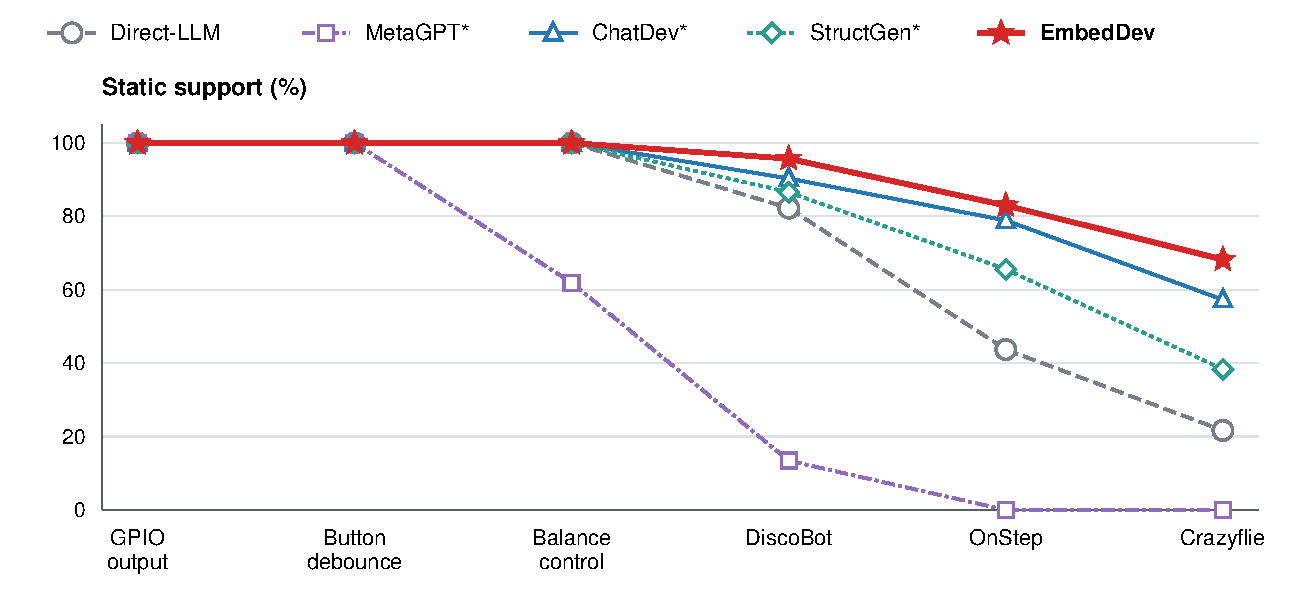
\includegraphics[width=\linewidth]{figures/rq3_static_support_six_tasks.pdf}
\caption{Assessment-assisted static support across six tasks (DeepSeek-V4-Pro; means over three repeats). * denotes adapted baselines.}
\label{fig:rq3-baseline-complexity}
\end{figure}

\paragraph{Local tasks provide limited separation.}
In the static view, all five methods reach 100\% support on GPIO output and button debounce. On balance control, \textsc{EmbedDev}, Direct-LLM, ChatDev, and StructGen also reach 100\%, while MetaGPT scores 61.90\%. Thus, small interfaces and bounded control requirements often leave little room to distinguish the methods on this static metric.

\paragraph{The advantage is clearer on multi-component tasks.}

In the static view, \textsc{EmbedDev} obtains the highest support on all three larger application tasks: 95.70\% on DiscoBot, 82.96\% on OnStep, and 68.22\% on Crazyflie. ChatDev is the strongest baseline on each, scoring 90.32\%, 78.89\%, and 57.28\%, respectively. The corresponding margins are 5.38, 4.07, and 10.93 percentage points. The updated RQ1 summary (Table~\ref{tab:rq1-method-model}) reports ChatDev's aggregate static support across these three application tasks as $75.50 \pm 1.26$\%, giving \textsc{EmbedDev} an aggregate advantage of 6.79 percentage points. StructGen scores 86.56\%, 65.56\%, and 38.33\%; Direct-LLM scores 82.26\%, 43.70\%, and 21.67\%; MetaGPT scores 13.44\%, 0\%, and 0\%.

The largest margin occurs on Crazyflie, whose requirements connect sensor acquisition, estimation, command selection, safety supervision, control, and motor outputs while preserving state and timing obligations. This pattern is consistent with design representations being useful when many behaviors must remain coordinated across functions and execution cycles. Nevertheless, \textsc{EmbedDev}'s 68.22\% support also exposes substantial remaining gaps. Task requirements and review granularity vary, and the advantage is not monotonic across the six tasks, so these results do not isolate a causal effect of complexity.

% rq3.tex
\begin{rqanswer}{3}
\textsc{EmbedDev} matches the static-assessment ceiling on the two GPIO tasks and leads static support on the three multi-component applications, with its largest observed advantage on Crazyflie. The benefit of design-centered generation is most apparent in the evaluated tasks with extensive coordination; this measure does not establish universal superiority or hardware correctness.
\end{rqanswer}
